%******************************************************************************************************
%*********************************** First Chapter ****************************************************
%******************************************************************************************************

\externaldocument{{../Chapter2/chapter2}}
\externaldocument{{../Chapter3/chapter3}}
\externaldocument{{../Chapter4/chapter4}}
\externaldocument{{../Chapter5/chapter5}}
\externaldocument{{../Chapter6/chapter6}}
\externaldocument{{../Chapter7/chapter7}}
\externaldocument{{../Appendix1/appendix1}}
\externaldocument{{../Appendix2/appendix2}}
\externaldocument{{../Appendix3/appendix3}}
\externaldocument{{../Appendix4/appendix4}}
\externaldocument{{../Appendix5/appendix5}}
\externaldocument{{../Appendix6/appendix6}}
\externaldocument{{../Appendix7/appendix7}}


\chapter{Introduction}  %Title of the First Chapter
\label{intro}

% **************************** Define Graphics Path **************************

\graphicspath{{Chapter1/Figs/}}


%TODO intro here? Describe what this chapter is for; background information
%TODO discuss fahim

The rest of this chapter is aimed at providing the reader with suitable background knowledge to provide context for this project and an understanding of the working environment. The last section of this chapter will outline the motivations for this project and the resulting objectives to be tackled in this project. 

%******************************************************************************************************
%******************************************************************************************************
\section{An Introduction to Unmanned Aerial Vehicles} 
\label{intro:UAVs}

The term Unmanned Aerial Vehicle (UAV) can be used to describe any form of aircraft that does not require a pilot on board. This term includes aircraft that are controlled remotely, autonomous vehicles capable of navigating themselves, and any aircraft that are a combination of the two. Other terms that may be familiar are ``drone'' and Unmanned Aerial System (UAS), which can be used interchangeably with UAV within the context of this project. 

UAVs come in a wide range of form factors but can be split into two main classes; fixed-wing UAVs and rotary wing UAVs. Fixed-wing UAVs are generally only capable of horizontal take-off and landing (HTOL), whilst rotary wing UAVs generally employ vertical take-off and landing (VTOL). There are, however, other forms of UAV which incorporate features of both main classes; for example, quadplane UAVS use rotary wing rotors to allow VTOL, but do the main bulk of their flying with forward facing rotors much like a fixed-wing UAV. Across these categories are a very wide range of UAV platforms, from hobbyist quadcopters to military attack vehicles, and many many others in between. %TODO images?  
Although the range of UAV form factors and their uses is vast, the vast majority are suitable for candidates for complete autonomous flight control, as shall be described in Section %TODO reference where we talk about adding hardware modules 
 
Although there were a large number of suitable candidates for the following work, it was decided that this project would be aimed at the control of strictly fixed-wing UAVs for the purposes of aerial photography. For that reason, we shall not discuss any other style of UAV. %TODO 

%******************************************************************************************************
%******************************************************************************************************
\section{UAVs for Aerial Photography} 
\label{intro:photography}

The first recorded use of aerial photography was in 1858 by a French balloonist and photographer known as ``Nadar'' at a height of 80 metres using a tethered hot air balloon. %TODO ref aerial photography history
Since then aerial photography has of course massively progressed, both in terms of the aerial vehicles in use and the cameras available. As such, it is now an activity that can be partaken in by both organisations, companies, and individuals alike, for a range of purposes. For example, aerial photography of course plays a very large role in intelligence gathering by government agencies and militaries, but can also be a hobby for otherwise earth-bound photography enthusiasts. 

Different applications will require different equipment and styles of photography; a hobbyist may want a wide panorama, whilst a mapping application will require a consistent vertical camera angle. The use of aerial photography for mapping or measurement is known as aerial photogrammetry, and will be the chosen field of interest for this project. Aerial photogrammetry is a specific subset of aerial photography in that it not only requires the capturing of images, but additional information about where the image was captured. For this project, we are looking at the use of aerial photogrammetry to create an image of the land below our UAV, either for mapping or general surveying purposes. In order to be able to do this, we need to be able to capture a set of images, and know the location of the UAV when the images were captured, to allow the images to be stitched together into one larger image of the ground beneath. In this scenario we can typically use GPS co-ordinates and a pre-planned imaging path to define which images relate to which areas of the ground below. %TODO refernce photogrammetry definition?


This project will primarily focus on the mapping of land beneath the UAV, and as such we need to define a specified flightpath over the chosen area. There are a number of typical flightpaths for surveying or mapping land, two forms are lawnmower pattern paths and spiral pattern paths. Fig. \ref{fig:simplelawnmower} shows the general form of a lawnmower pattern, and Fig. \ref{fig:simplespiral} shows us the general form of a spiral pattern.

\begin{figure}[htbp!] 
\centering    
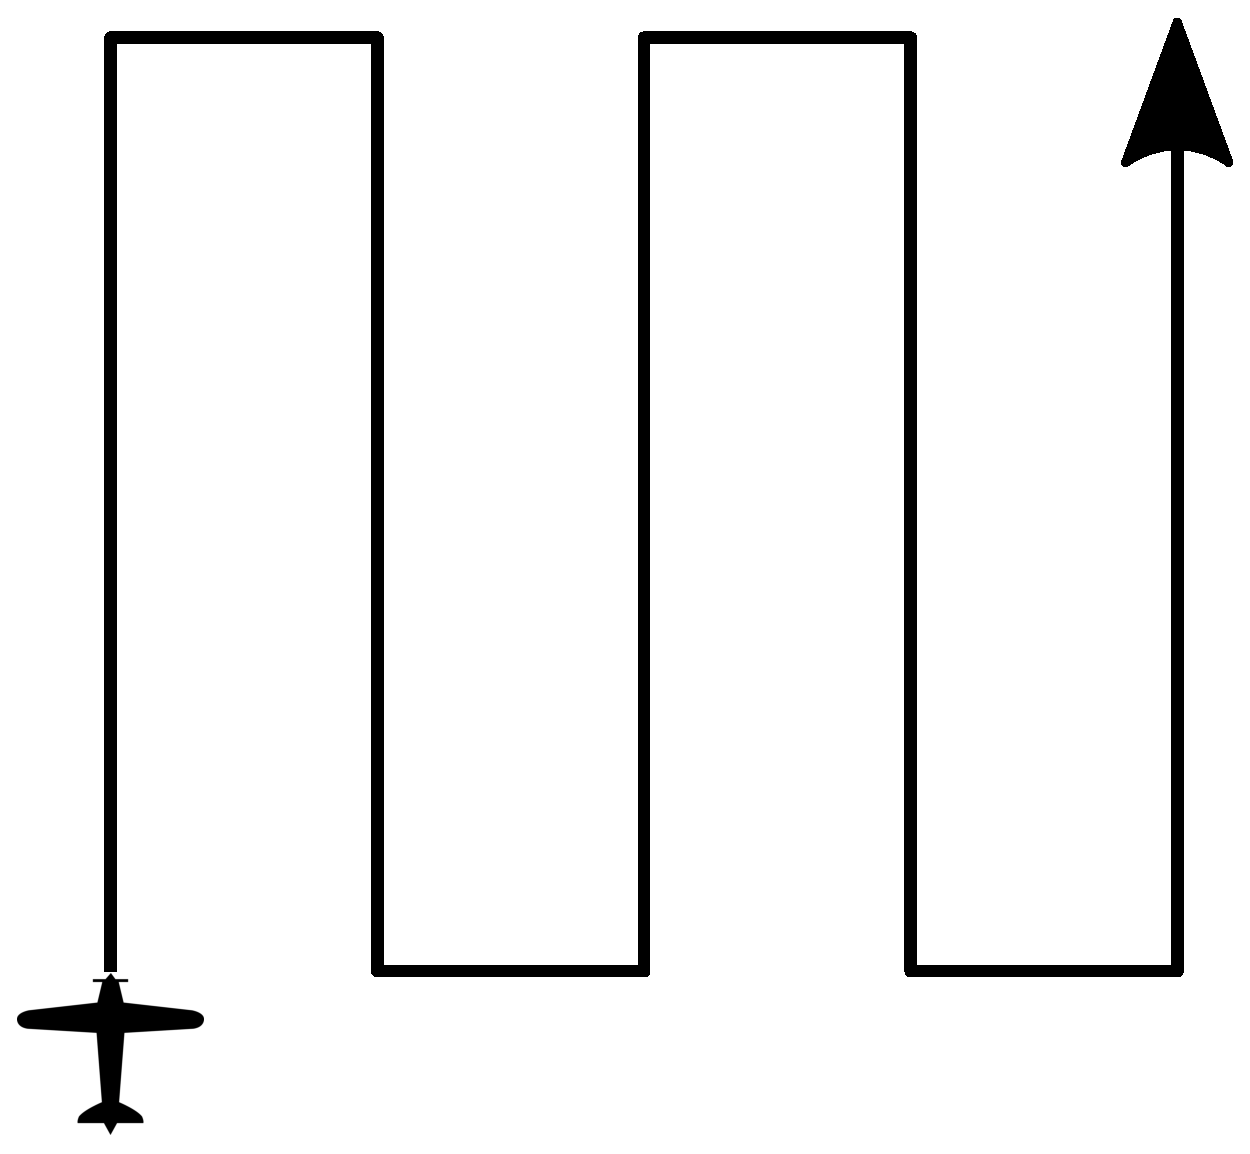
\includegraphics[width=0.7\textwidth]{SimpleLawnmower}
\caption[Simple Lawnmower Pattern]{The general form of a lawnmower pattern aerial imaging flightpath}
\label{fig:simplelawnmower}
\end{figure}

\begin{figure}[htbp!] 
\centering    
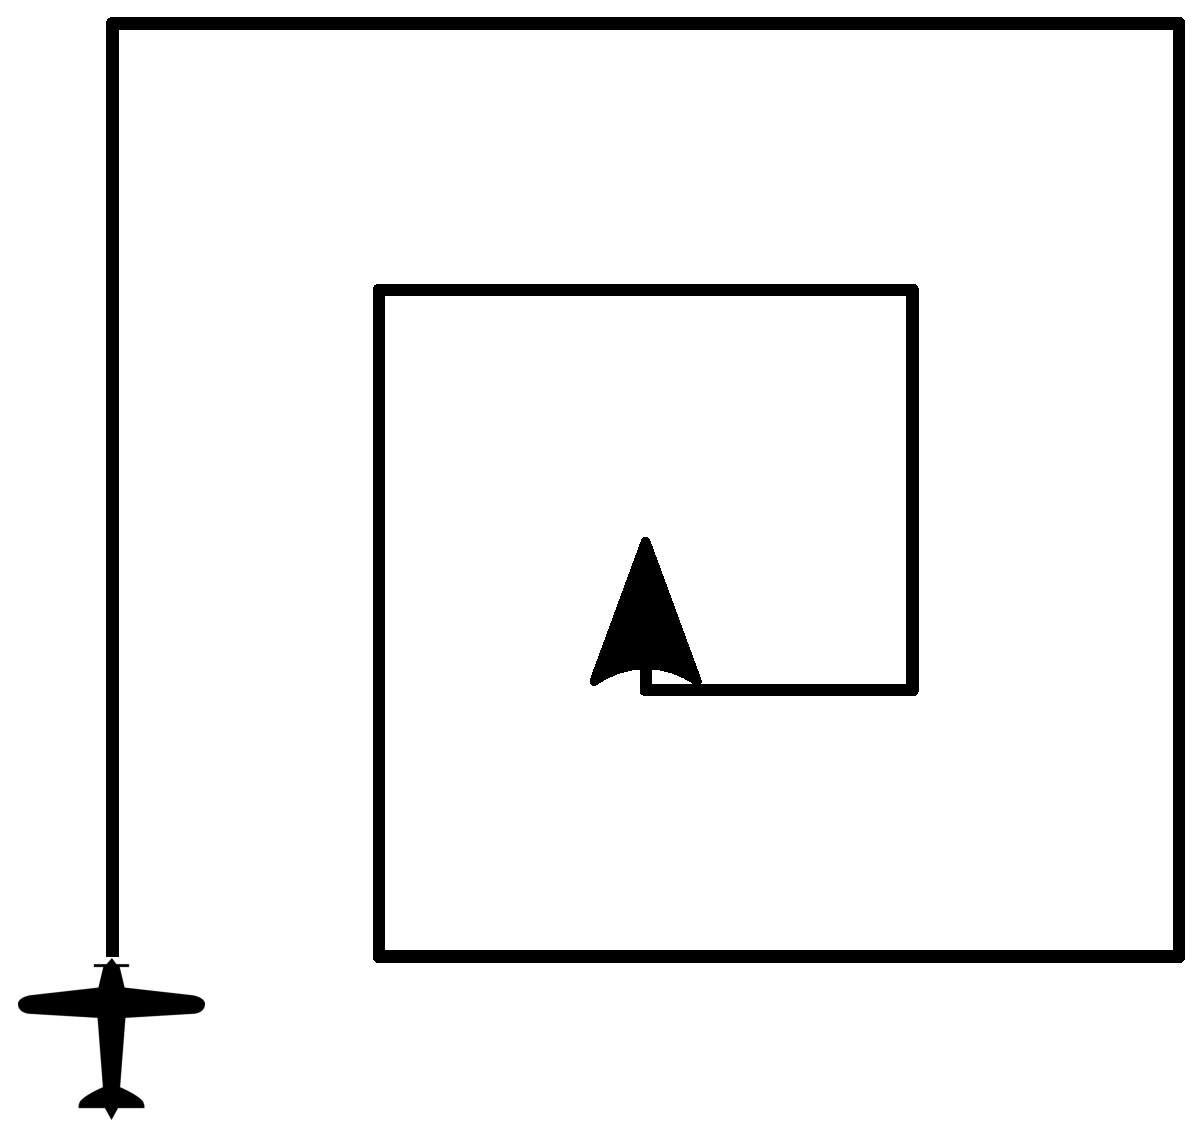
\includegraphics[width=0.7\textwidth]{SimpleSpiral}
\caption[Simple Spiral Pattern]{The general form of a spiral pattern aerial imaging flightpath}
\label{fig:simplespiral}
\end{figure}

Using these patterns, we can define what shall be referred to henceforth as ``imaging paths'' or ``imaging runs''. These are the sections of the flightpath for which we are capturing images of the ground below, and as such we very much care about the position and orientation of the UAV whilst following these paths. For the lawnmower pattern the imaging paths are the vertical sections of the path seen in Fig. \ref{fig:simplelawnmower}, whereas for the spiral path all sections of the flight plan are considered imaging paths. 

As the lawnmower pattern does not require the horizontal sections of the path in Fig. \ref{fig:simplelawnmower} to be used for capturing images, we are not particularly concerned with how we fly between the imaging paths. Knowing this, we can specify our flightpath in terms of simply our imaging paths, as can be seen in Fig. \ref{fig:imaginglawnmower}

\begin{figure}[htbp!] 
\centering    
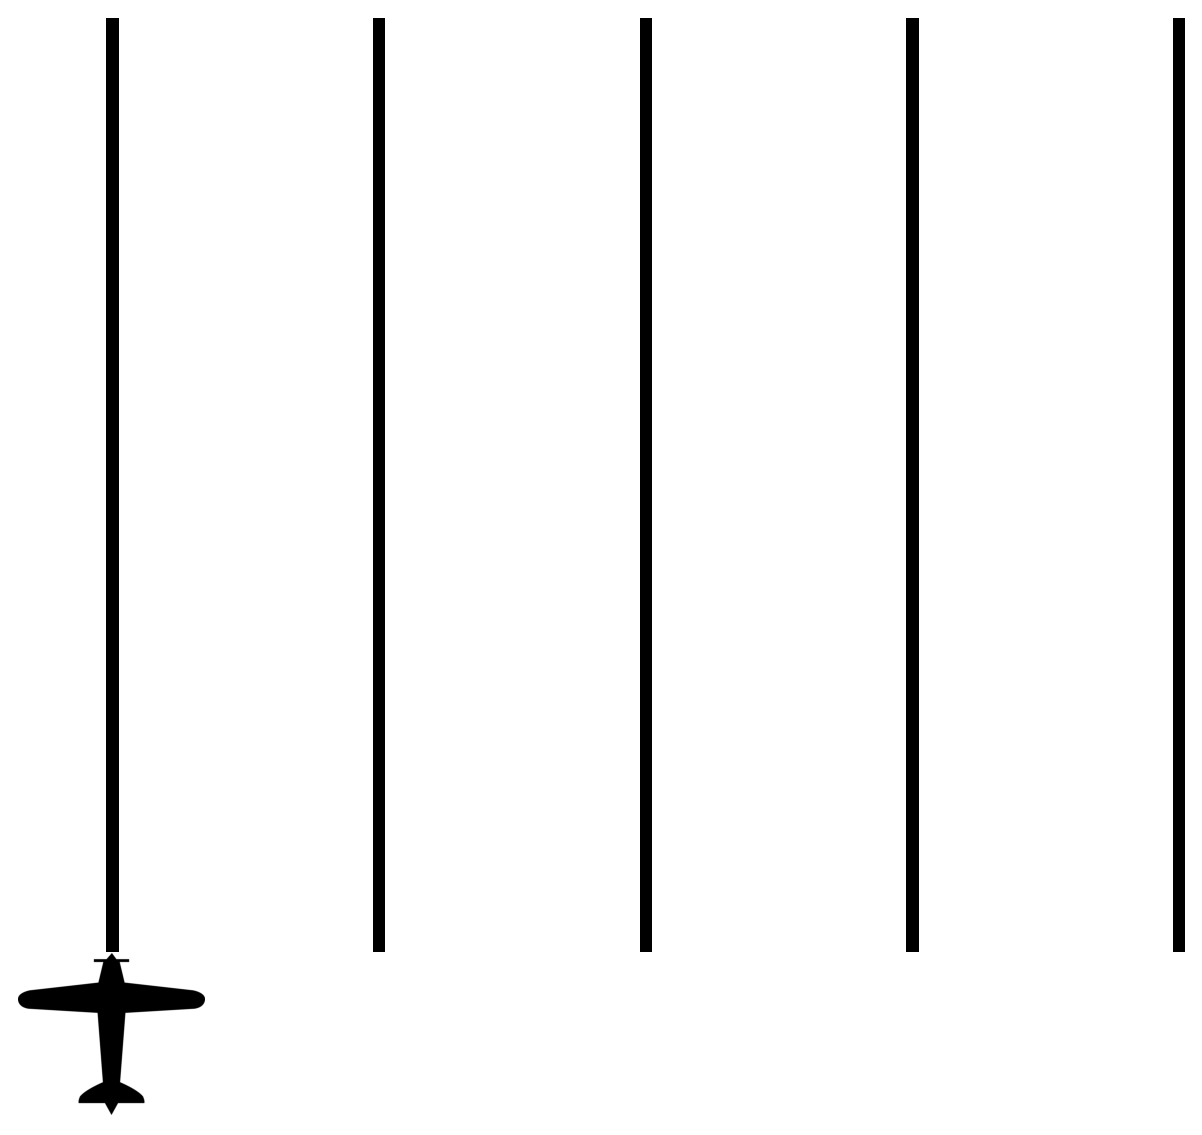
\includegraphics[width=0.7\textwidth]{ImagingLawnmower}
\caption[Imaging Lawnmower Pattern]{A version of the lawnmower pattern, using only imaging paths}
\label{fig:imaginglawnmower}
\end{figure}

As the imaging paths shown in Fig. \ref{fig:imaginglawnmower} are separate of one another, it is possible to complete each imaging path in any order and in either direction. This does however require the user to plan accordingly and to record location data accurately so as to be able to stitch together the resulting photographs correctly. One of the resulting patterns that we can create from this is called the ``Zamboni pattern'', named after the route a Zamboni machine takes around an ice rink to smooth out the ice. A Zamboni pattern describes a path whereby we d onot traverse up and then down adjacent imaging paths, but instead perform a series of overlapping paths by travelling up one imaging path, and then down a path a few rows over. This is necessary for a Zamboni due to its large minimum turning radius, and would be equivalent to a UAV with a large turning radius being required to traverse a number of very close imaging paths. 

The required flightpath will have to be calculated based on a number of factors including:
\begin{itemize}
	\item The size of the area we are wishing to photograph
	\item Changes in ground elevation over the chosen area
	\item The operational range of the UAV based on battery life or fuel amount
	\item The desired resolution of the resulting images - we must fly lower for higher detail images
	\item The distance between imaging paths will be a function of the desired flying height and the angle of the lens on the camera
	\item The path to follow between the imaging paths will be a function of the turning performance of the UAV
	\item Environmental factors such as wind during the flight
\end{itemize}

These factors shall be considered and discussed later in this report where relevant, and have been used to inform decisions throughout the work of this project.

Throughout this work we shall be referring to a flightpath as a ``mission'', which describes a full, pre-planned flight path from take-off to landing. To define these missions we require particular software products that shall be discussed in Section \ref{intro:planner}.



%TODO finalise
%TODO define mission planning process in this section

%******************************************************************************************************
%******************************************************************************************************
\section{ArduPilot} 
\label{intro:ardupilot}

ArduPilot, also known as ArduPilotMega (APM), is an open-source suite of autopilot products aimed at hobbyists and professionals alike. ArduPilot includes the ArduPlane, ArduCopter, and ArduRover autopilots, each aimed at aeroplane style UAVS, helicopter and multirotor UAVS, and ground based rover platforms respectively. As previously mentioned, this project is aimed at fixed-wing aeroplane UAVs, and as such this report is looking at the ArduPlane product. 

ArduPilot has been around since late 2009 and was originally designed to operate using the Arduino development ecosystem. Since then, the codebases have evolved in both size and functionality, in part due to hardware improvements which will be discussed in \ref{intro:planner}. This has lead to both the software and hardware components of these ArduPilot autopilot solutions moving away from Arduino almost entirely.

ArduPilot grew out of an organisation called DIYDrones, %TODO ref DIYDrones.com
which was set up as an online community for enthusiasts to discuss and create solutions for UAV use; this community still exists and operates as one of the many hubs for discussion regarding UAVs, autopilots, and route planning. In 2014, the group of people maintaining the ArduPilot project teamed up with The Linux Foundation to create a non-profit organisation called the Dronecode Project. The Dronecode Project is an effort to collaborate a number of open-source hardware and software products under one structure, which includes the ArduPilot project. In February 2016, it was announced that the core team behind ArduPilot would be creating their own non-profit organisation to best suit the needs of the users of the ArduPilot products, however at the time of writing this is still a work in progress. %TODO ref dronecode, non-profit announcements, linux foundation

\subsection{ArduPlane}
\label{intro:arduplane}

ArduPlane is designed so that when paired with a suitable controller board (see Section \ref{intro:hardware}), it enables autonomous flight on almost any fixed-wing UAV. %TODO ref http://ardupilot.org/plane/index.html 
To do this, the ArduPlane software is compiled to create the firmware, which is then programmed onto the controller board alongside the mission plan. Once the controller board is connected to all of the necessary control outputs and sensor inputs, the UAV must be configured and tuned for flight, and then is ready for take-off. The configuration and tuning are of course capabilities provided by ArduPlane, however are not relevant for discussion within the context of this project. ArduPlane handles both automatic take-off and landings, as well as providing the option to change between flight modes. The flight modes available include fly-by-wire modes, an acrobatics mode, a training mode, and an automatic flight mode. For this project we are only concerned with the automatic flight mode, and shall not be dealing with any other mode. 

The ArduPlane codebase uses a very large collection of libraries, of which the majority are also used by the ArduCopter and ArduRover products. This, combined with the fact that ArduPlane is designed to work with any fixed-wind UAV means that a lot of the code is very generic and reusable. The codebase for the whole ArduPilot project currently consists of roughly 11,000 files in total, and the specific ArduPlane code (excluding any shared libraries or resources) is made up of only 37 files. The sheer number of shared files, generic coding style, and open-source nature of this project combine to mean that in many respects the code commenting and documentation is very lacking and unspecific. That being said, there are a number of instructional guides and references that can be found on the ArduPilot website for anyone looking to modify the code or get involved with contribution. In addition to this, there are a number of forums that can provide many answers to common problems. %TODO ref diydrones, discuss.ardupilot.org, and apm forum	
In addition to there being three main autopilot platforms, there are also a large number of differing released versions and code branches, which are often platform specific or hardware specific.

%TODO finish?


\subsection{JSBSim}
\label{intro:jsbsim}

As the ArduPilot project is open source, there are a number of associated open-source utilities available to download for testing purposes. One of the main tools used in ArduPlane development is called JSBSim, an open-source Flight Dynamics Model (FDM) which can be used as part of a flight simulator. %TODO ref jsbsim.sourceforge.net

We are able to use this FDM to provide a Software In The Loop (SITL) simulator, which does not require any additional hardware besides a computer. This enables us to modify the ArduPilot code and test it with a range of flight missions without the need to purchase a control board or have a suitable UAV available. 

The ArduPlane project includes a utility to simulate and view a fixed-wing UAV in flight, starting at any given GPS location. Fig. \ref{fig:jsbsim} shows one example of this, where we have the command window, an output console, and a map view. The map view shows us the planned mission and the actual path the UAV will follow in the given scenario, the console window displays output and communication messages from the UAV, and the command window allows us to control the simulator.

\begin{figure}[htbp!] 
\centering    
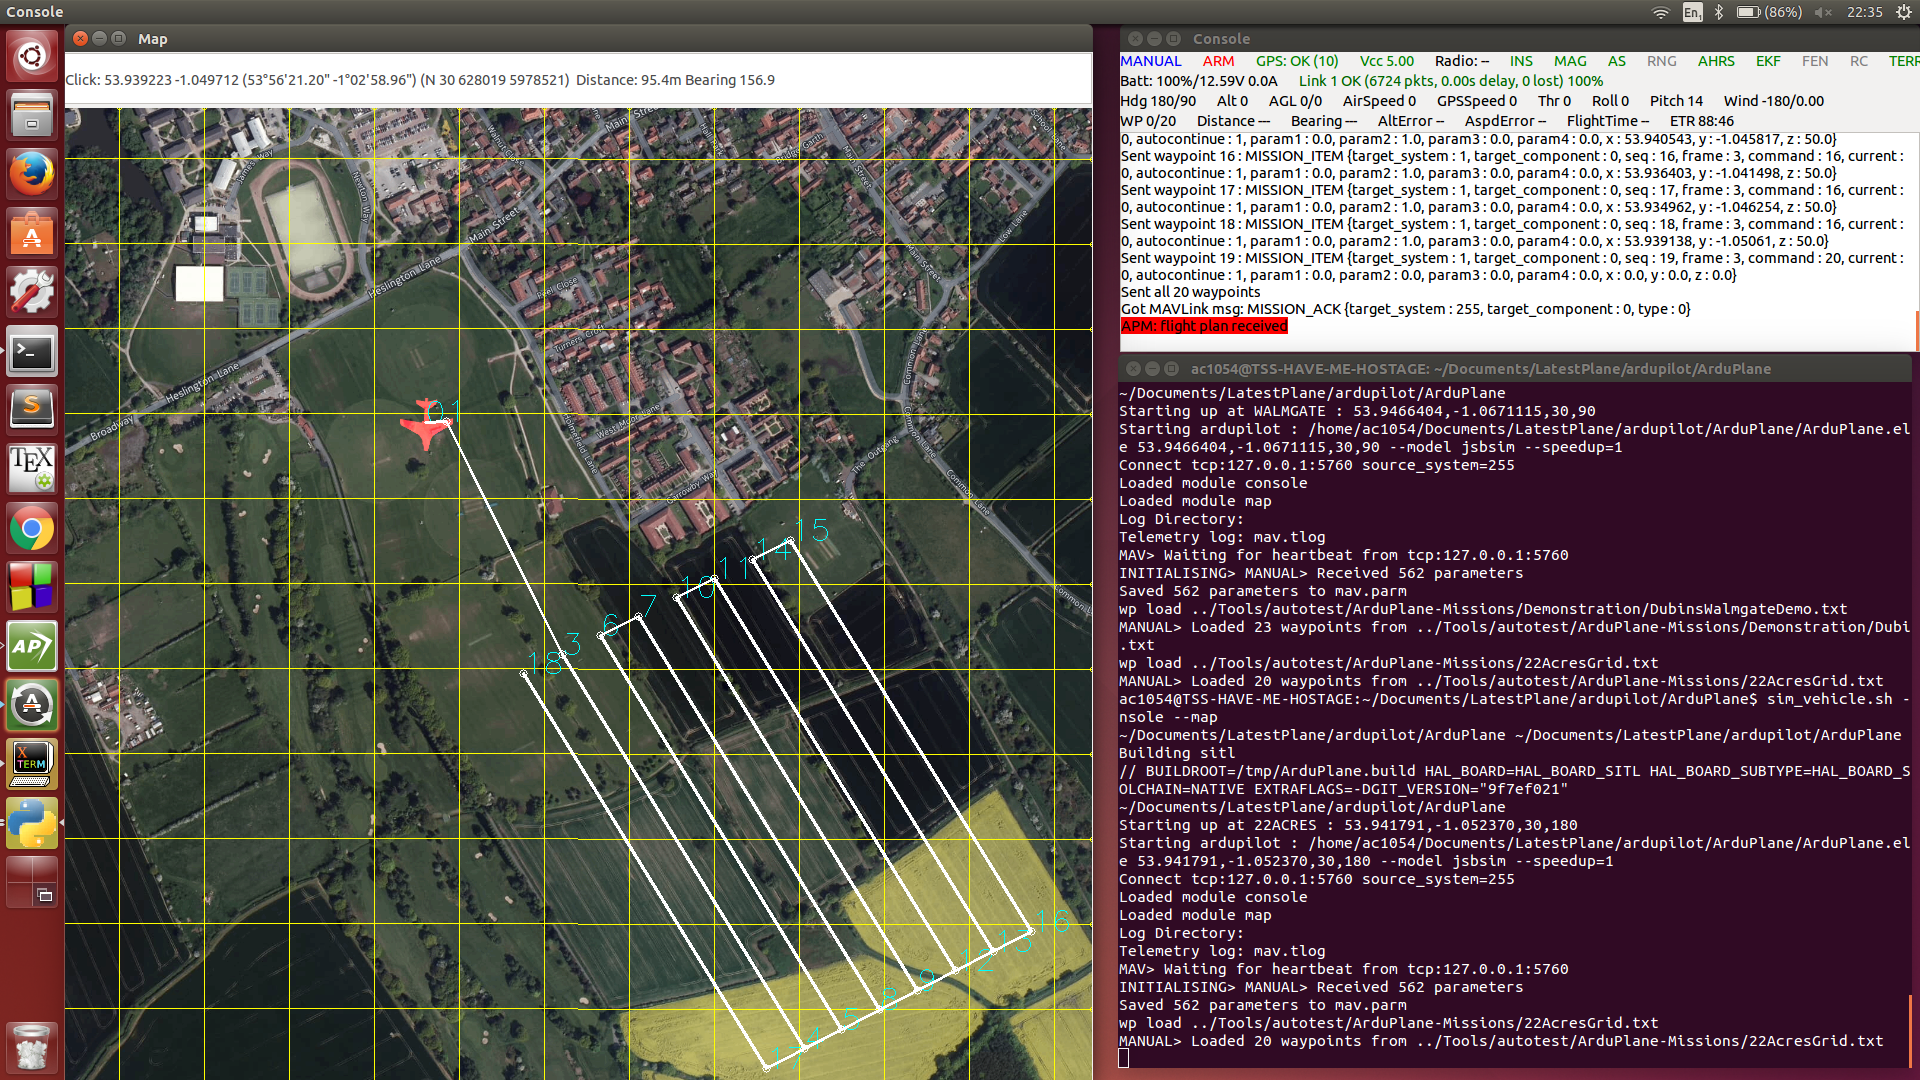
\includegraphics[width=\textwidth]{JSBSim}
\caption[JSBSim Simulator]{A view of the JSBSim based flight simulator, showing a command window, output console, and simulator map view}
\label{fig:jsbsim}
\end{figure}

This simulator forms the bulk of the testing for this project, and is used to map flight paths and record performance. Each simulated UAV flight generates a log in the form of a \textit{.BIN} file. We can then use the MAVExplorer utility and our ground control software to analyse the log files. 

\subsubsection{MAVExplorer}
\label{intro:mavexplorer}
MAVExplorer is a log analysis tool, provided in the form of a python script suitably named \textit{MAVExplorer.py}. This allows us to generate a map of the area over which the UAV has flown with white lines displaying the planned mission, and a green line plotting the actual route the UAV flew. An example of this can be seen in Fig. \ref{fig:mavexplorer}.

\begin{figure}[htbp!] 
\centering    
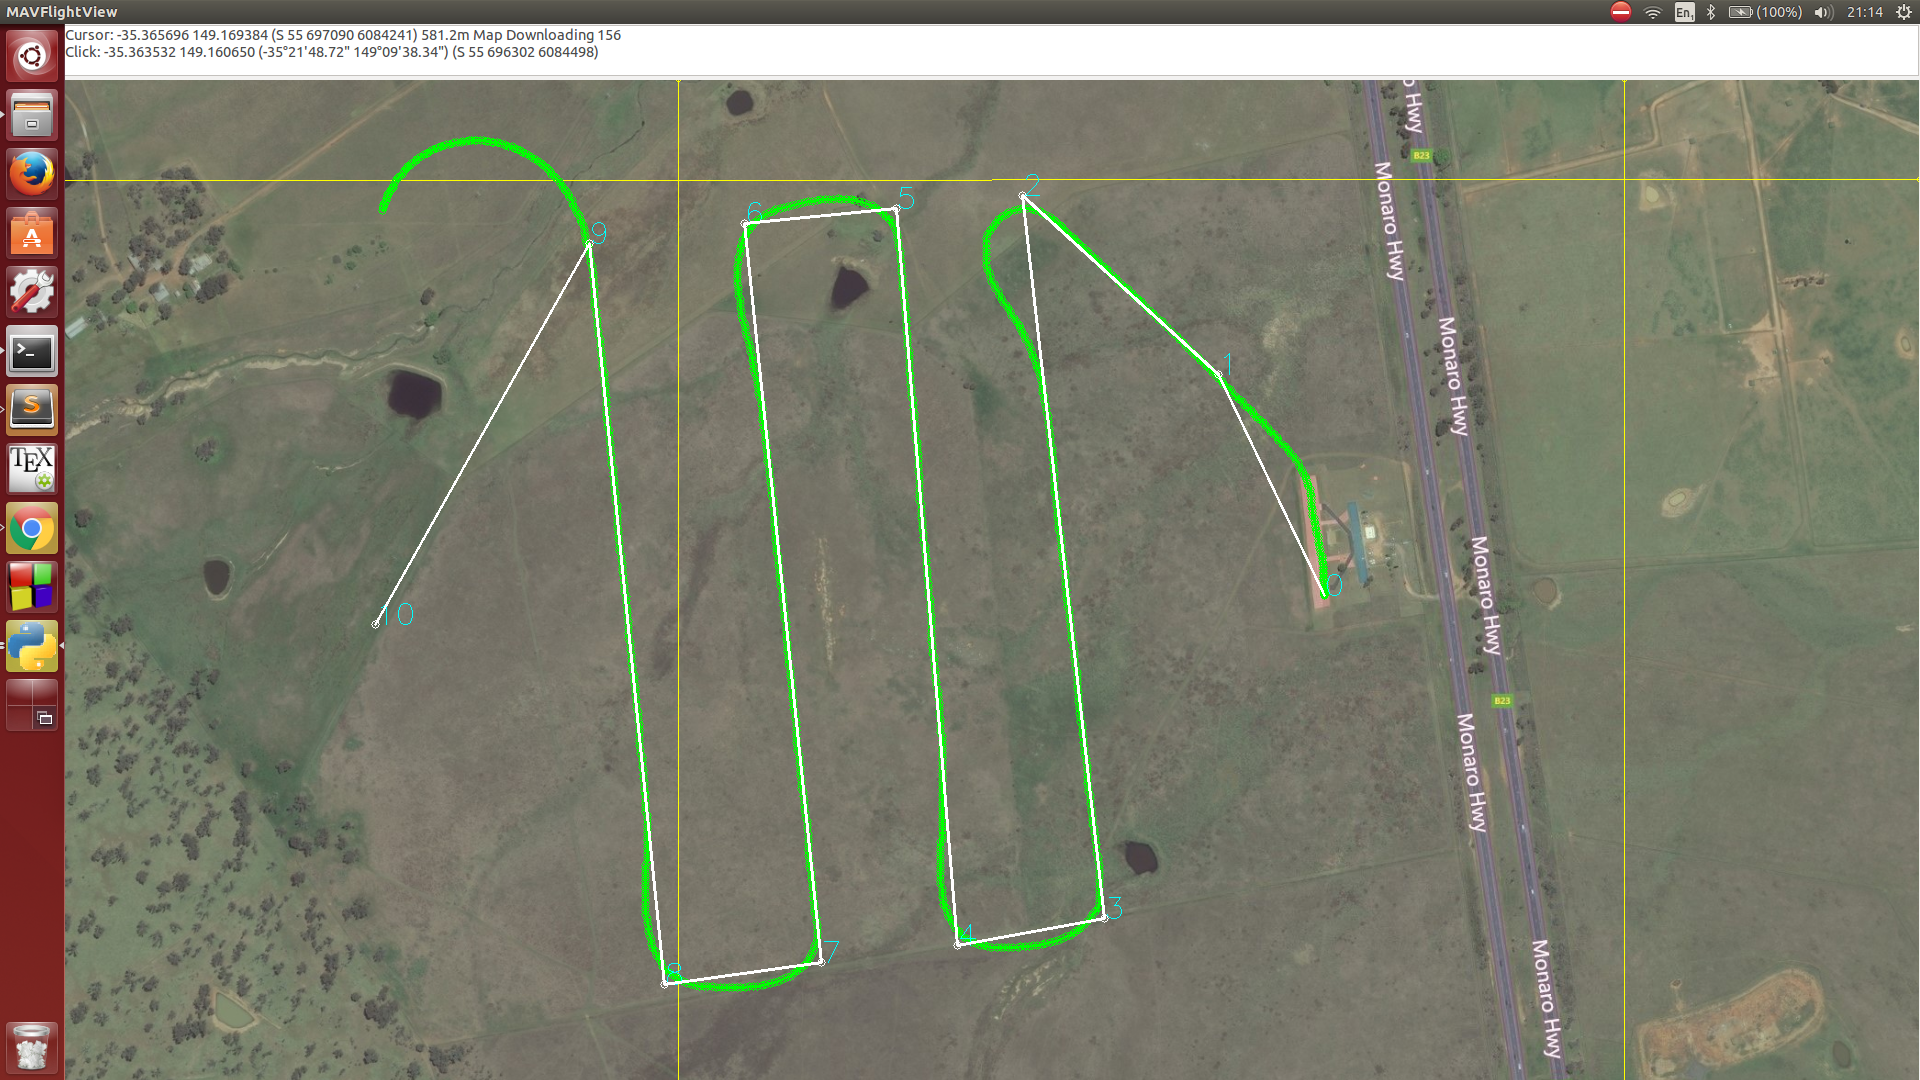
\includegraphics[width=\textwidth]{MAVExplorer}
\caption[MAVExplorer Example]{The mapping view provided by MAVExplorer utilising log files from flight simulations}
\label{fig:mavexplorer}
\end{figure}

\subsection{MissionPlanner and APM Planner}
\label{intro:planner}

As previously mentioned, for autonomous UAV flight we need to plan out a mission before flight. There are a number of software products capable of this, however the main two used by the ArduPilot project are called APM Planner 2 and MissionPlanner. Both of these products are open source however APM Planner 2 runs on Linux, Windows, and Mac OSX, whilst MissionPlanner is a Windows only application. Both products enable mission planning however the MissionPlanner product is more feature rich, reliable, and quick to use. 

The missions plans generated using either of these programs are of the same format; a text file with a number of commands, parameters, and often GPS locations. This is very useful as it allows manual editing of these text files where necessary, and allows us to easily work out how the autopilot itself reads its commands from the provided mission plan. 

There are a wide range of commands that can be included in a mission including take off commands, land commands, and navigation commands. For this project the most relevant navigation commands are those conducted using waypoints. We are able to instruct he UAV to loiter around a point at a specified radius for a number of rotations (complete circles around a point), a duration, or indefinitely. The other form of navigation command is simply an instruction to travel to a point in space, with the option to define how close to that point we need the UAV to travel. 

Fig. \ref{fig:missionplanner} shows a typical mission plan in MissionPlanner, where we are commanding a simple lawnmower pattern imaging run. 

\begin{figure}[htbp!] 
\centering    
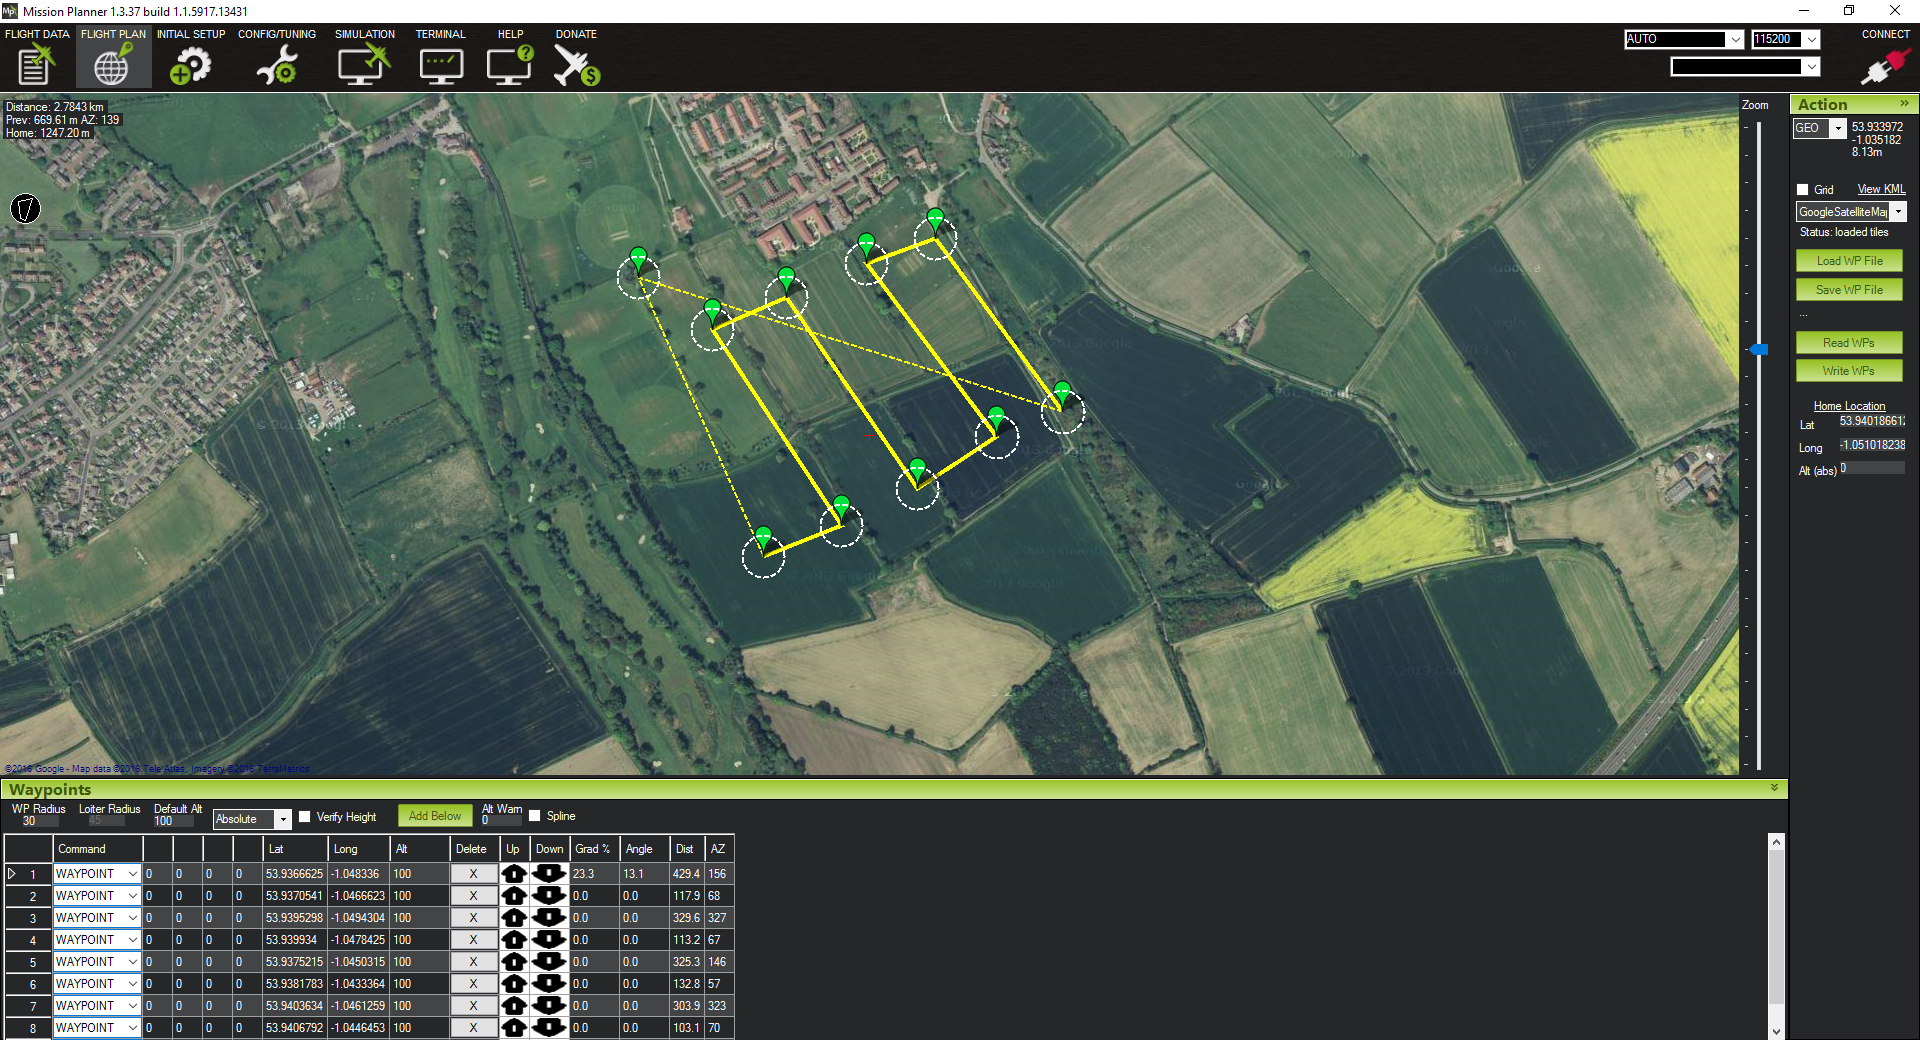
\includegraphics[width=\textwidth]{MissionPlanner}
\caption[MissionPlanner Desktop Software]{The mission planning view of the Windows based MissionPlanner software}
\label{fig:missionplanner}
\end{figure}

%******************************************************************************************************
%******************************************************************************************************
\section{Autopilot Hardware} 
\label{intro:hardware}

As also mentioned, one of the key components for autonomous UAV flight using ArduPlane is the controller board which must be mounted on the UAV itself. There are a number of currently available boards that ArduPilot can run on, and over the years there have been many versions of these. These control boards are responsible for processing the mission plan and controlling the aircraft accordingly. During flight, the control board uses GPS readings alongside other sensor readings where available to direct the aircraft. It does this using the servos connected to the control surfaces, and controlling the thrust generated from the propeller(s) or engine(s). The control board can be connected other devices too, such as camera gimbals and parachute release devices, however these are not in use throughout this project. 

There are currently 4 supported controller boards that have open hardware design, and 4 controller boards with closed hardware designs. Additional to this are a number of controller boards which are no longer supported, as they do not have the storage capabilities to load on the latest versions of the code. The most popular currently supported board is the Pixhawk board, which can be seen in Fig. \ref{fig:pixhawk}, and has an open hardware design. The APM 2.x series of controller boards, seen in Fig. \ref{fig:apm2}, used to be very popular however are no longer supported for the latest versions of the code.

\begin{figure}[htbp!] 
\centering    
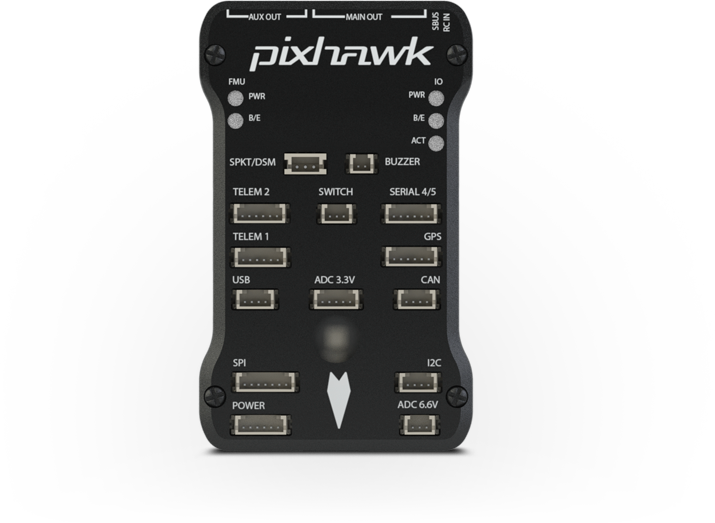
\includegraphics[width=0.6\textwidth]{Pixhawk}
\caption[Pixhawk Controller Board]{The Pixhawk controller board, for which the hardware specification and design is openly available, from \cite{Pixhawk}}
\label{fig:pixhawk}
\end{figure}

It is possible to still use the APM 2.x boards as they are still available for purchase online and will work with older versions of the ArduPlane code. This may be beneficial in certain situations, as the Pixhawk board is considerably more expensive than an APM board. The presence of a controller board is not essential for this project, as we are able to use the SITL simulator described in Section \ref{intro:jsbsim} to simulate UAV flight without one. If one is present, it is possible to use a Hardware In The Loop (HITL) simulator to test changes to the codebase by running them on a controller board. In this instance, the controller board replaces JSBSim whilst simulating flight.

\begin{figure}[htbp!] 
\centering    
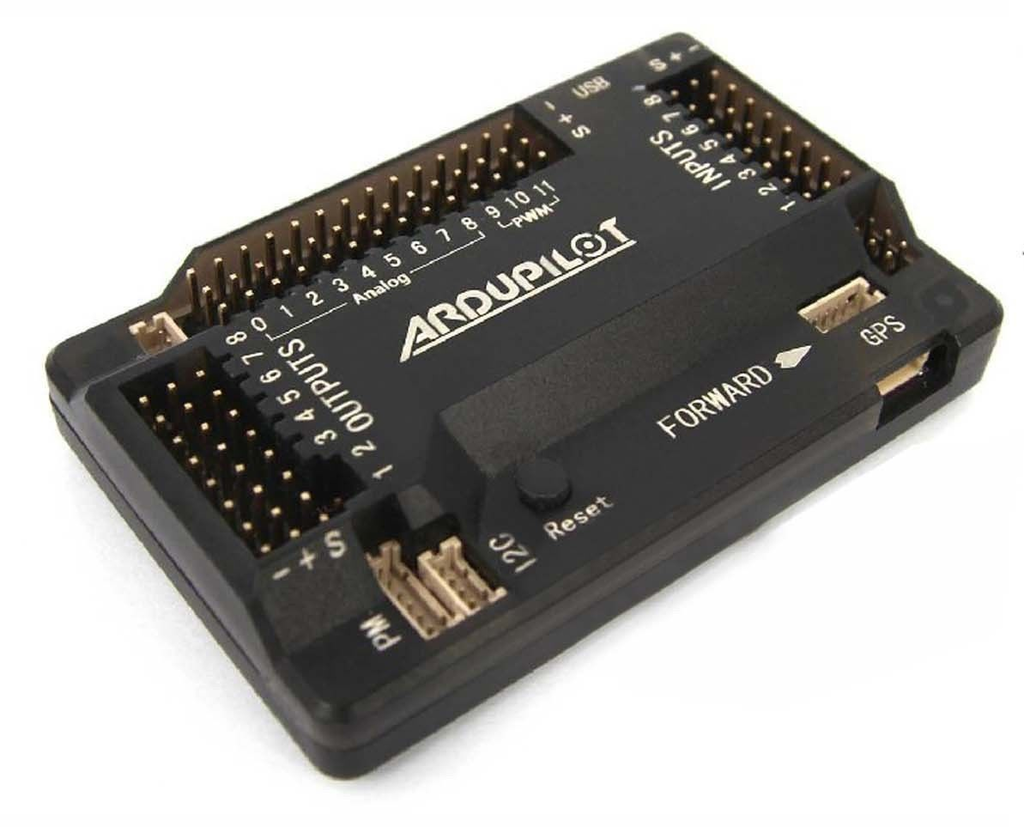
\includegraphics[width=0.5\textwidth]{APM2}
\caption[APM 2.6 Controller Board]{The APM 2.6 controller board, which is no longer supported by the ArduPilot project, from \cite{Apm2}}
\label{fig:apm2}
\end{figure}

%******************************************************************************************************
%******************************************************************************************************
\section{Project Motivations and Objectives} 
\label{intro:objectives}

The inspiration for this project comes from its supervisor, Dr Andrew Pomfret. He was part of an expedition to map a glacier in Svalbard, Norway using a UAV equipped with a camera in order to determine any movement of the glacier over time. Although using a professional grade UAV and associated route planning software, he found a number of its features lacking. The most relevant issue was that planning a battery efficient route that would also capture high quality images was laborious, and that regardless of how well you planned the route, he felt the UAV would often not be optimising its battery usage. Following lengthy discussion between the author and Dr Pomfret, two primary objectives were defined.

\subsection{Objective 1: Efficient Route Planning}
\label{intro:obj1}
Our first objective is to implement an efficient method for route planning. The solution should enable a user to plan a route that allows us to deliver high quality aerial photographs, without using more battery power than is required. When discussing high quality aerial photographs, we are talking primarily about the position of the UAV relative to the planned route above ground, and as such we require the UAV to be commanded to follow the imaging paths described in Section \ref{intro:photography}. This requires us to plan a route which will result in the UAV travelling the full length of the imaging path which in turn requires the UAV to be aligned with the imaging path before starting it. 

A further requirement for this task is that the planning method should be user-friendly and calculate a desired route from standard waypoint definitions provided in the mission planning software.

Building on these aims, it is necessary for this system to work for flight in any environment, meaning it must be able to plan a route that works for the UAV in windy conditions. As such we must incorporate knowledge of the flying environment when planning the path, be that in real-time when flying or beforehand when plannig, this shall be explored later.

\subsection{Objective 2: Route Following}
\label{intro:obj2}

Our second objective follows on from our first objective, and requires us to enable the UAV to fly the newly define path types. This will require modification of the ArduPlane code so as to be able to understand any new commands and perform them as desired. This may also require a new method of path following than is currently available in official versions of ArduPlane. 

Additionally, this objective should work with the first to provide flight in windy conditions. This may be entirely a feature of the planning stage or it may be a feature of the autopilot implementation, this shall be explored later.
%TODO finalise objectives

